\section{State of the art} \label{sota}

\subsection{Taxonomy}

It is certainly useful to start with a review of the different ways to categorize the features and algorithms used by researchers in the field of radio frequency fingerprinting. More specifically, we'll focus on Radio Frequency Machine Learning (RFML) research, though other fingerprinting techniques exist that don't involve machine learning. The goal is to define our needs precisely and select the important factors to consider.

\subsubsection{Taxonomy for features} \label{features_tax}

The features we select must allow us to identify a precise device among potentially very similar devices. We need what \textcite{delgado_passive_2020} describe as a Physical Unclonable Function (PUF). PUFs are physical distortions that are unique to a specific system. They are another way of talking about fingerprints.

\textcite{xu_device_2015} propose three ways to categorize radio signal features:

\begin{itemize}
  \item based on the specificity of the feature (from vendor specific to device specific),
  \item based on the layers (PHY, MAC, Network and higher),
  \item and based on the acquisition method (passive or active).
\end{itemize}

Features from the MAC and higher layers typically require in depth knowledge of the protocols in play. Not only that, but they also tend to be less specific than we would like (either vendor specific or depending on the type of device). This indicates we should probably focus on the physical (PHY) layer features, which rely on imperfections in the manufacturing process of the devices.

\subsubsection{Taxonomy for fingerprinting algorithms} \label{algo-taxo}

\textcite{riyaz_deep_2018} provide a visual categorization of fingerprinting approaches, which we adapt in figure \ref{fig:algo-taxo}. We take a look at these approaches in the following paragraphs.

\begin{figure}[htp!]
  \centering
  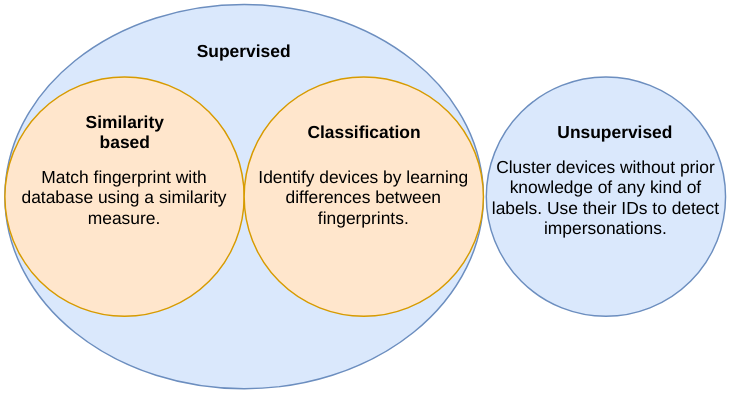
\includegraphics[scale=0.5]{figures/sota_algo-taxonomy.png}
  \caption{Fingerprinting algorithms taxonomy}
  \label{fig:algo-taxo}
\end{figure}

\paragraph{Supervised approaches:} Supervised approaches use features from labelled data to generate a function capable of separating the different classes. These approaches can be further categorized in similarity based and classification techniques.

Similarity based techniques are white-list algorithm that use a database of fingerprints and a similarity measure to determine whether a device is legitimate. Developing a technique like this usually requires prior knowledge of vendor specific device features \cite{riyaz_deep_2018}.

Classification systems can also require deep knowledge of the features and protocols used, in the case of "traditional", manually tuned classifiers. Those are built to extract predetermined features and work similarly to other white-list algorithms afterwards.

In this age of deep learning though, research seems to be more interested in classification techniques that are able to extract the features they need by themselves. This can be done through deep Multi-Layer Perceptrons (MLP) \cite{delgado_passive_2020, stankowicz_complex_2019} or through more advanced techniques like Convolutional Neural Networks (CNN) \cite{riyaz_deep_2018, oyedare_estimating_2019, youssef_machine_2017, morin_transmitter_2019, sankhe_no_2019}. The latter have proved very powerful in domains like computer vision, natural language processing and recommendation systems. This success is one of the reasons experimentations on CNNs are common in RFML research.

\paragraph{Unsupervised systems:} Unsupervised approaches cannot by themselves discriminate a legitimate device from an illegitimate one. They don't have that information, since they work with unlabeled data. In order to detect attempts of impersonation, such a system has to keep a record of fingerprints and linked identifiers (MAC addresses, serial numbers...). It can then throw an alert and update a black-list when multiple fingerprints are linked to the same ID or when multiple IDs are linked to the same fingerprint \cite{xu_device_2015, nguyen_device_2011}.

\textcite{xu_device_2015} specify that unsupervised approaches are appropriate when the fingerprints of legitimate devices are not available.

% -------------------------------------------------------------------------------------------------------------
\subsection{Acquisition}

The vast majority of the research considered for this project uses USRP systems to record transmissions as raw I/Q signals. The number of devices can be anywhere from 5 to 500 (but most often less than 20). They all use data acquired from WiFi (802.11) or Zigbee (802.15.4) devices. \cite{riyaz_deep_2018, oyedare_estimating_2019, youssef_machine_2017, morin_transmitter_2019, sankhe_no_2019, nguyen_device_2011}

Some, like \textcite{sankhe_no_2019}, also describe how they add artificially induced impairments to simulated signals with MatLab. This is something we could also do, but it is secondary. The focus is on the creation of a robust dataset of real world transmissions between an NFC reader and tags.

% -------------------------------------------------------------------------------------------------------------
\subsection{Features}

\subsubsection{Features selection}

Even if we don't plan to manually select and extract the features that will form the fingerprints of our devices, it is useful to learn about them. It will allow us to make sure they are present for the algorithm to extract and also allow us to design preprocessing methods that magnify the features.

Whether we end up with a system that is able to identify many devices uniquely, or one that only tries to separate a specific device from the others, we will need device specific accuracy. We don't want to make relay attacks impossible only if the attacker doesn't use a device from the same vendor as the victim's device. This is why in section \ref{features_tax}, we concluded that the features we are most interested in are from the physical layer.

Because of their nature, these features should be appropriate no matter the protocol used. The following list is composed of features described by \textcite{riyaz_deep_2018} and also used in other works.

\begin{itemize}
  \item{I/Q imbalance:} The amplitude and the phase are not exactly the same on the in-phase and the quadrature signals, because of the imperfections in the quadrature mixers.
  \item{Phase noise:} When the baseband signal is up-converted to the carrier frequency, it is sensible to phase noise which creates rotational vibrations.
  \item{Carrier frequency offset:} The difference between the carrier frequency of the transmitter and the carrier frequency of the receiver.
  \item{Harmonic distortions:} The Digital-to-Analog Converters (DAC) cause harmonic distortions because of imperfections.
\end{itemize}

\subsubsection{Preprocessing}

It is clear that preprocessing the data appropriately can greatly increase the accuracy of a model and reduce its complexity.

The first question to ask is how should the data be partitioned, in order to be fed to the learning algorithm. This question will be discussed in section \ref{nn-architecture} since it is identical to choosing the input of our model.

Several works mention wavelet transforms (either discrete or continuous) as effective means to amplify the characteristic features of a wireless device \cite{xu_device_2015, oyedare_estimating_2019, youssef_machine_2017}. They report increased accuracy and scalability, and reduced complexity. It is certainly worth it to explore this preprocessing method.

% -------------------------------------------------------------------------------------------------------------
\subsection{Machine learning applied to radio frequency}

\subsubsection{Challenges} \label{challenges}

\textcite{riyaz_deep_2018} highlight some of the challenges faced when working on RFML problems. They are reformulated in the three first items of the list below. The next items are personal additions.

\begin{enumerate}
  \item \label{itm:chall1} Finding the optimal partition length to feed the learning algorithm.
  \item \label{itm:chall2} Finding the optimal network architecture for the problem (in the case of neural networks).
  \item \label{itm:chall3} The absence of standard datasets to train and evaluate a model.
  \item Finding a cheap preprocessing method that improves performance and reduces complexity.
  \item Achieving a demonstrably scalable system.
\end{enumerate}

Great insight into item \ref{itm:chall1} is given by \textcite{youssef_machine_2017}. Indeed, they compare the performance of models trained with different input segment sizes. We delve deeper into this matter as well as item \ref{itm:chall2} in section \ref{nn-architecture}.

Item \ref{itm:chall3} is the core matter of the first part of our project. Indeed a considerable portion of our work consists in the elaboration of a dataset of NFC transmissions for different PICC devices.

\subsubsection{Supervised or unsupervised}

The aim of this project is to explore supervised learning techniques. This is why most of the literature considered here studies supervised systems. Also, in general, it seems works that use supervised methods are a lot more abundant than their unsupervised counterparts. This could be because of the popularity of models such as convolutional neural networks, and their apparent adaptability to the problem of RF fingerprinting.

Despite this, we can see that unsupervised learning techniques are also showing promising results. An example of this is the work of \textcite{nguyen_device_2011}. The paragraph about unsupervised systems in section \ref{algo-taxo} describes the basics of their system pretty well. They use a Nonparametric Bayesian model to detect the number of devices and then cluster them based on their fingerprints. This technique allows them to discriminate between an unknown number of devices that the model never encountered before. They show good results with four devices using two features strictly from the PHY layer.

While this work is interesting, it uses pre-engineered features. We were unable to find research on deep unsupervised learning techniques (such as deep belief networks) for the problem. Such a solution could be an interesting topic for another project.

\subsubsection{Comparing supervised approaches}

Several articles have compared the performance of different machine learning approaches. In the next paragraphs we discuss the findings of two of them.

\textcite{riyaz_deep_2018} compared their Convolutional Neural Network (CNN) with the techniques of Support Vector Machine (SVM) and logistic regression. They report substantially higher performance using their CNN (up to 60-70\% better accuracy). Their results, although limited in the number of devices (they only classify up to five), also seem to show that CNNs are more scalable than the other methods. Indeed, increasing the number of classes caused a significant drop in the performance of the other algorithms, but not for the CNN.

\textcite{youssef_machine_2017} compare the performance of four supervised algorithms: SVM, Deep Neural Networks, CNN and Accelerated Levenberg-Marquardt Multi-Stage Training (A-LM MST). The latter is an advanced classification technique that makes training deep neural networks less resource heavy by using a hierarchy of smaller Multi-Layer Perceptrons (MLP) rather than one big MLP. They use data collected from 12 WiFi transmitters.

Their results show impressive performance for their MST, especially when provided with very little data. Their CNN model is close second, although it performed significantly worse with very little data. Then comes the DNN with pretty good results and then only the SVM.

These results can guide us in our choices of experimentation. They show that SVM algorithms, while capable to some extent, are not appropriate for this specific problem. They also show CNNs are very promising, more scalable and more adaptable than "simple" DNNs. The MST solution is very interesting, but reducing the computational complexity is not our primary concern and the improvement doesn't seem that substantial.

\subsubsection{Neural network architectures} \label{nn-architecture}

In section \ref{challenges}, we noted that one of the challenges we face is to find the optimal partition length for the input of our model. To give an element of answer, \textcite{youssef_machine_2017} don't only compare the performance of 4 different models, they also do it with five different partition sizes (32, 64, 128, 256 and 512). They find their DNN architecture handles short segments better than long ones, while their CNN gets progressively more performant as the segments get larger.

\textcite{stankowicz_complex_2019} compare different kinds of formats for their inputs: two real valued series (one for the I component and one for the Q component), one complex valued series and one complex valued series with a spectrogram added as additional information. Their results are not the clearest, but they seem to show better performance when using a single series of complex values as input. They also show better performance in general for models that use complex valued weights. This is an interesting argument that we could explore.

Another of the challenges previously noted is finding the optimal architecture for a neural network in the context of RF fingerprinting. Studying the various architectures employed in previous works can help us define what is effective and what direction to take for our own experiences. We won't describe specific architectures in this section, but will reference elements from them when conceiving our experiments.

In general, the works cited throughout this section train their models to output the ID of a specific device. In this project, we would like to try training our model to simply discriminate between a legitimate device and the others. Elements like incremental learning (the ability to train the model again with more devices without starting from zero) and shift invariance (the ability not to care about the position of values in the input) are also important to take into consideration.
